\documentclass[11pt,a4paper]{article}
\usepackage[utf8]{inputenc}
\usepackage[T1]{fontenc}
\usepackage{booktabs, amsmath, amssymb, natbib, listings, xcolor, enumitem, parskip, geometry, hyperref, bm}
\usepackage{tikz}
\usetikzlibrary{shapes.geometric,arrows.meta,positioning,fit,backgrounds,calc}

\geometry{margin=1in}
\setlength{\parskip}{3pt}

\definecolor{codeblue}{RGB}{30,100,200}
\definecolor{layerA}{RGB}{210,230,255}
\definecolor{layerB}{RGB}{210,255,220}
\definecolor{layerC}{RGB}{245,220,255}
\definecolor{layerD}{RGB}{255,235,210}
\lstset{
  basicstyle=\ttfamily\small,
  keywordstyle=\color{codeblue}\bfseries,
  commentstyle=\color{gray},
  breaklines=true,
  frame=single
}

% -----------------------------------------------------------------------
\title{\textbf{Two Brains, One Network: Dual-Process Topology Management\\
for Heterogeneous Physics-Informed Kolmogorov-Arnold Networks}}
\author{
  Richard Liu \quad Yufei Zou \\
  School of Data Science \\
  University of North Carolina at Charlotte \\
  \texttt{github.com/RicardoLaMo/OpKAN}
}
\date{March 2026}

\begin{document}
\maketitle

% -----------------------------------------------------------------------
\begin{abstract}
Physics-informed Kolmogorov-Arnold Networks (KANs) introduce a structural management
problem that gradient descent cannot solve: when should an edge remain a B-spline, be
replaced by a symbolic function, or be pruned? We formalize this as the \emph{topology
surgery problem} and show that it creates five chronic failure modes in heterogeneous
KANs: topology stagnation, parameterization lock-in, symbolic-numerical tension, regime
blindness, and instability in the second-derivative smoothness required by the PDE. To
address this, we propose a \textbf{dual-process topology agent}: a fast reflexive
controller performs high-frequency local maintenance such as pruning and learning-rate
stabilization, while a slow strategic controller performs low-frequency topology surgery
guided by PDE geometry and market-regime signals. A typed DSL, static AST allowlist, and
atomic rollback ensure that every mutation preserves twice-differentiable smoothness
($C^2$ continuity) and transactional integrity. We demonstrate the framework on a Heston
stochastic-volatility PI-KAN, where stable second derivatives are a hard requirement
because of the cross-derivative term. An ablation shows that System~2 is required for
regime-ordered behavior, while System~1 restores full throughput; PDE residual
minimization alone fails all five financial monotonicity checks under distributional
shift, revealing a broader training-objective insufficiency in physics-constrained
learning under regime change. The system sustains $\mathbf{26{,}300}$\,smp/sec on H200
with zero GPU blocking, showing that online structural governance need not compromise
training efficiency.
\end{abstract}

\medskip
\noindent\textbf{Keywords:} Kolmogorov-Arnold Networks, Physics-Informed Neural Networks, Dual-Process Architecture, Topology Management, Heston Stochastic Volatility, Options Pricing, Large Language Models, Heterogeneous Neural Networks

% =====================================================================
\section{Introduction}
\label{sec:intro}
% =====================================================================

\subsection{Problem: The Topology Surgery Problem}

A Kolmogorov-Arnold Network (KAN) places learnable activation functions on
\emph{edges} rather than nodes, which means the network is a mutable mathematical
object: any edge can be a B-spline, replaced by a closed-form symbolic function, or
pruned to zero during training. This edge-level replaceability is what makes KANs
attractive for physics-informed settings---it allows domain knowledge to be injected
directly into the network's mathematical structure.

However, it also creates a problem that gradient descent cannot solve. Gradient descent
can optimize the coefficients of a B-spline edge, but it cannot decide that the edge
should \emph{switch class}: from spline to symbolic form, or from a weak edge to zero.
A near-zero activation has a near-zero gradient, so the edge persists indefinitely
consuming computation. A B-spline that happens to approximate $\sin(x)$ remains a
B-spline indefinitely, losing interpretability and efficiency. We call this the
\textbf{topology surgery problem}: a class of structural decisions that falls strictly
outside the scope of gradient-based optimization.

This problem manifests in five distinct failure modes, each arising from a specific
gradient-signal gap---a setting where the training loss provides no corrective signal
for the structural decision that must be made:

\begin{enumerate}[nosep]
  \item \textbf{Topology stagnation.} Near-zero B-spline edges persist through training
  because their loss gradient is also near-zero. The edge contributes nothing but
  continues consuming computation.

  \item \textbf{Parameterization lock-in.} Gradient descent has no incentive to change
  an edge's parameterization class. A B-spline approximating $\sin(x)$ remains a
  B-spline indefinitely, losing interpretability and efficiency.

  \item \textbf{Symbolic-numerical tension.} Symbolic edges have no trainable parameters.
  In a mixed topology, gradient cannot flow through symbolic edges to inform neighboring
  B-spline adaptations, creating dead zones in the optimization landscape.

  \item \textbf{Regime blindness.} Under distributional shift (market regime change), a
  frozen topology cannot adapt. Weight updates shift the learned function but cannot
  restructure which edges carry which mathematical primitives.

  \item \textbf{$C^2$ instability.} Aggressive learning-rate updates can make an edge
  insufficiently smooth for stable second-derivative computation. In the Heston setting,
  the PDE contains a cross-derivative term $\rho\sigma vS\,\partial^2 V/\partial S\partial v$
  evaluated by autograd, so unstable edge curvature propagates as NaN.
\end{enumerate}

\subsection{Our Approach: Dual-Process Topology Agent}

The five problems decompose naturally by frequency and cognitive type. Problems~1 and~5
(topology stagnation and $C^2$ instability) are high-frequency and low-complexity: they
can be detected from local statistics and handled with simple actions such as pruning or
learning-rate adjustment. These are reflexive maintenance tasks; a fast model ($<$50\,ms,
7B parameters) is sufficient.

Problems~2, 3, and~4 (parameterization lock-in, symbolic-numerical tension, and regime
blindness) are low-frequency and high-complexity. They require reasoning about global
activation geometry, the mathematical validity of candidate symbolic forms, and the
relationship between market regime and topology adaptation. A slower, larger model
(200--500\,ms, 32B parameters) is needed for this multi-step mathematical reasoning.

A single fast model makes mathematically incoherent symbolic replacements. A single slow
model blocks the GPU. The \textbf{dual-process design} is not merely an efficiency
tradeoff; it follows from the structure of the problem itself. Reflexive maintenance and
strategic topology surgery are different kinds of decisions that should not be collapsed
into a single controller.

We evaluate this framework on a Heston stochastic-volatility PI-KAN, where $C^2$
continuity, PDE geometry reasoning, and real-time regime adaptation impose hard
correctness requirements that expose dual-process advantages invisible in unconstrained
settings.

\subsection{Contributions}

\begin{enumerate}[nosep]
  \item A taxonomy of five chronic management problems in heterogeneous KAN topology,
  each mapped to a specific gradient-signal gap, and a demonstration that they decompose
  across two cognitive timescales.

  \item A \textbf{dual-process topology agent} (System~1/System~2) that addresses all
  five failure modes, with the two paths operating concurrently without GPU blocking.

  \item A \textbf{typed DSL} with AST allowlist and atomic rollback providing type
  safety, vocabulary restriction ($C^2$ continuity preserved by construction), and
  transactional integrity.

  \item \textbf{Evaluation on Heston options pricing} with the key finding that PDE
  residual minimization alone fails all five financial monotonicity checks under
  distributional shift---a training-objective insufficiency result that may extend to
  other physics-constrained networks.
\end{enumerate}

% =====================================================================
\section{Related Work}
\label{sec:related}
% =====================================================================

\textbf{KANs and symbolic regression.}
The KAN architecture \citep{liu_etal_2024_kan} places learnable activations on edges,
grounded in Kolmogorov's superposition theorem \citep{kolmogorov1957representation}.
Symbolic edge replacement exists in the original library but is manual and offline;
our contribution is making it online and agent-driven under formal invariants.

\textbf{Physics-informed neural networks and finance.}
PINNs \citep{raissi2019physics} embed differential operator residuals in the training
loss. Financial applications \citep{horvath2021deep} have used MLP backbones; the
$C^2$ continuity required by the Heston cross-derivative term has received limited
attention, motivating our B-spline edge design.

\textbf{LLM agents and dual-process AI.}
Kahneman's fast/slow framework \citep{kahneman2011thinking} motivates the two-speed
design. Toolformer \citep{schick_etal_2023_toolformer} and ReAct \citep{yao_etal_2023_react}
use LLMs as tool orchestrators over stateless API calls; our agent manages the
continuous evolution of a heterogeneous mathematical object under formal invariants,
a fundamentally different task.

\textbf{Regime detection.}
Hamilton's HMM \citep{hamilton1989new} is our backbone for market regime identification.
The regime-blindness failure mode (Problem~4) shows why a topology agent must be
regime-aware; PDE loss alone does not impose behavioral ordering across Heston parameter
regimes.

\textbf{Neural architecture search.}
NAS \citep{elsken2019neural} automates topology discovery offline. Our agent operates
online, on a running network, with natural language input and domain-specific mathematical
constraints---complementary to NAS for initialization, but a distinct runtime concern.

% =====================================================================
\section{Methods}
\label{sec:methods}
% =====================================================================

\subsection{Data}

\textbf{Options data.} We use OPRA options data for SLV (iShares Silver Trust ETF).
The live benchmark uses a single quote date for cross-sectional evaluation; the replay
benchmark replays a historical sequence of silver/regime feature data with a replayed
SLV surface template to evaluate performance across regime transitions over time.

\textbf{HMM features.} The regime detector consumes five time-series features computed
from market microstructure: (1)~log-return $\ell_t$, (2)~realized volatility
$\hat{\sigma}_t$ (20-bar window, annualized), (3)~implied volatility $\sigma^\text{IV}_t$,
(4)~IV--RV spread $\Delta_t = \sigma^\text{IV}_t - \hat{\sigma}_t$, and (5)~IV momentum
$\mu^\text{IV}_t = \sigma^\text{IV}_t - \sigma^\text{IV}_{t-1}$.

\textbf{Collocation points for PDE training.} The PI-KAN is trained on randomly sampled
collocation points $(S, v, t)$ drawn uniformly from $[0,200]\times[0,0.5]\times[0,1]$
and normalized to $[0,1]^3$ before being passed to the network. Interior points are used
to evaluate the Heston PDE residual; boundary points are used to enforce the terminal
payoff and boundary conditions.

\textbf{Model families evaluated.} Six model configurations are compared:
\texttt{bs\_plain} (Black-Scholes with baseline ATM volatility),
\texttt{bs\_regime} (Black-Scholes with HMM regime-predicted volatility),
\texttt{rf\_direct} (random forest direct price prediction),
\texttt{spikan\_hybrid} (symbolic PI-KAN residual + regime-vol BS anchor),
\texttt{spikan\_plain\_hybrid} (symbolic PI-KAN residual + plain-formula BS anchor), and
\texttt{spikan\_plain\_iv\_hybrid} (plain-formula anchor + learned IV-space residual,
our headline model).

\subsection{Physics-Informed KAN (PI-KAN)}

\textbf{Why KAN over MLP.} Standard MLP activations (ReLU) produce zero second
derivatives, making the Heston cross-derivative term $\rho\sigma vS\,\partial^2 V/\partial S\partial v$
numerically degenerate when evaluated via autograd. KAN's B-spline edges---cubic splines
with \texttt{grid\_size=5} and \texttt{spline\_order=3}---are $C^2$ continuous by
construction, providing well-defined second derivatives throughout training.

\textbf{The Heston PDE.} Option fair value $V(S,v,t)$ satisfies:
\begin{equation}
\frac{\partial V}{\partial t}
+ \frac{1}{2}vS^2\frac{\partial^2 V}{\partial S^2}
+ \rho\sigma vS\frac{\partial^2 V}{\partial S\partial v}
+ \frac{1}{2}\sigma^2 v\frac{\partial^2 V}{{\partial v}^2}
+ rS\frac{\partial V}{\partial S}
+ \kappa(\theta-v)\frac{\partial V}{\partial v}
- rV = 0
\label{eq:heston_pde}
\end{equation}
with boundary conditions: $V(S,v,T)=\max(S-K,0)$ (terminal payoff), $V(0,v,t)=0$
(zero spot), and $V(S,v,t)\approx S - Ke^{-r(T-t)}$ as $S\to\infty$.

\textbf{Training loss.} The composite loss minimizes PDE residual plus boundary error:
\begin{equation}
\mathcal{L} = \underbrace{\mathbb{E}_{\bm{x}\sim\Omega}\!\left[\left|\mathcal{N}[V](\bm{x})\right|^2\right]}_{\mathcal{L}_\text{PDE}}
+ \lambda_\text{BC}\underbrace{\mathbb{E}_{\bm{x}\sim\partial\Omega}\!\left[\left|V(\bm{x})-V_\text{target}(\bm{x})\right|^2\right]}_{\mathcal{L}_\text{BC}}
\label{eq:loss}
\end{equation}
where $\mathcal{N}[V]$ is the Heston differential operator evaluated via
\texttt{torch.autograd} with \texttt{create\_graph=True}.

\textbf{Architecture.} OpKAN uses a $[3,16,1]$ configuration (inputs $(S,v,t)$, 16-node
hidden layer, scalar output $V$). Three edge types coexist at runtime:
\texttt{BSplineEdge} (8 basis functions, trainable coefficients + SiLU base),
\texttt{C2SymbolicEdge} (closed-form expression from the 20-function AST allowlist, no
trainable parameters), and \texttt{ZeroEdge} (returns \texttt{torch.zeros\_like(x)},
implementing correct prune semantics).

\subsection{Hidden Markov Regime Detector}

A Gaussian HMM with $K=3$ states and diagonal covariance is fit on the five market
microstructure features above. Walk-forward inference uses non-overlapping 20-day
windows, refitting from scratch at each boundary. The HMM produces regime label
$r_t\in\{0,1,2\}$ at each step, where states are sorted by mean realized volatility
to ensure label~0 always maps to the lowest-volatility regime across rolling windows
(label stability fix). This label feeds System~2's context for strategic topology
decisions. A detected regime transition triggers a strategic query even if fewer than
100 training steps have elapsed.

\subsection{Dual-Process Topology Agent}

The five failure modes decompose by cognitive timescale. Problems~1 and~5 (stagnation,
$C^2$ instability) are high-frequency: detectable from local statistics, resolvable with
threshold rules. Problems~2, 3, and~4 (parameterization lock-in, symbolic-numerical
tension, regime blindness) are low-frequency but require multi-step mathematical
reasoning over global network structure and PDE geometry.

\textbf{System~1 (Reflexive, $<$50\,ms, Qwen 2.5-7B).}
Every 10 training steps, the training loop places (step index, per-edge L1 norms,
recent loss delta) into a bounded queue (\texttt{maxsize=1}). A background thread
invokes the 7B model, which produces a \texttt{ReflexDecision}:

\begin{lstlisting}[language=Python]
class ReflexDecision(BaseModel):
    reasoning: str       # brief justification
    prunes: List[str]    # edge IDs with L1 norm below threshold
    lr_adjustment: float # multiplier in [0.5, 2.0]
\end{lstlisting}

The 7B model handles pattern recognition (is this norm below 0.005?), not deep
reasoning. This path addresses Problems~1 (stagnation) and~5 ($C^2$ instability).

\textbf{System~2 (Strategic, 200--500\,ms, Qwen 2.5-32B).}
Every 100 training steps, a longer-horizon context (loss trajectory, HMM transition
probabilities, full KAN topology state, regime signals) is placed in a separate bounded
queue. A second background thread invokes the 32B model, which produces a
\texttt{StrategicDecision}:

\begin{lstlisting}[language=Python]
class StrategicDecision(BaseModel):
    reasoning: str                    # structural reasoning over PDE geometry
    mutations: List[EdgeMutation]     # REPLACE, PRUNE, or KEEP per edge
    regime_analysis: RegimeThesis     # HMM transition diagnosis
    training_command: Literal["CONTINUE", "HALT"]
\end{lstlisting}

The 32B model is necessary because edge replacement decisions require: (a) identifying
that an activation profile approximates a specific smooth function, (b) verifying the
candidate formula is $C^2$ on its natural domain, and (c) reasoning about how the
replacement interacts with the Heston cross-derivative term. These are multi-step
mathematical tasks that 7B models perform unreliably. This path addresses
Problems~2, 3, and~4.

\textbf{Non-blocking coordination.}
The \texttt{EngineCoordinator} manages four bounded queues (two input queues,
\texttt{maxsize=1}; two output queues, \texttt{maxsize=32}). At the start of each
training batch, \texttt{apply\_pending\_mutations()} non-blockingly drains both output
queues. If no decisions are pending, training continues at full GPU throughput. The GPU
never waits on the LLM.

\begin{figure}[ht]
\centering
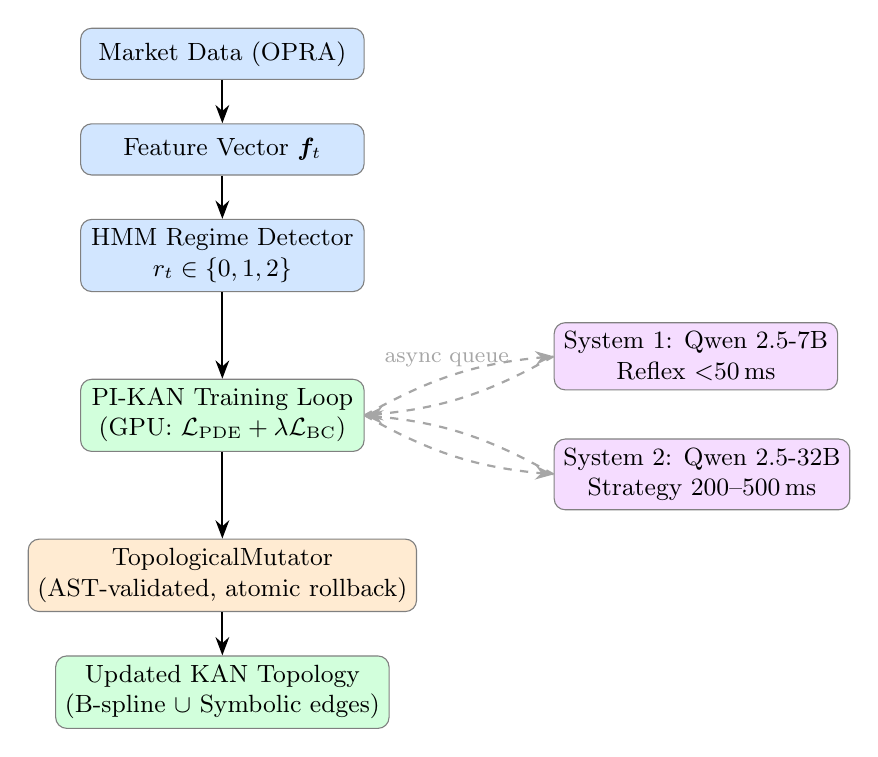
\begin{tikzpicture}[
  node distance=0.55cm and 2.2cm,
  box/.style={rectangle, rounded corners=4pt, draw=black!50, minimum width=3.6cm,
              minimum height=0.65cm, align=center, font=\small},
  databox/.style={box, fill=layerA},
  kannbox/.style={box, fill=layerB},
  agentbox/.style={box, fill=layerC},
  secbox/.style={box, fill=layerD},
  arr/.style={-Stealth, thick},
  dasharr/.style={-Stealth, dashed, thick, gray!70}
]
%% ---- Data column (left) ----
\node[databox] (market)   {Market Data (OPRA)};
\node[databox, below=of market]  (feat)    {Feature Vector $\bm{f}_t$};
\node[databox, below=of feat]    (hmm)     {HMM Regime Detector\\$r_t \in \{0,1,2\}$};
%% ---- PI-KAN (centre) ----
\node[kannbox, below=1.1cm of hmm] (pikan)
  {PI-KAN Training Loop\\(GPU: $\mathcal{L}_\text{PDE}+\lambda\mathcal{L}_\text{BC}$)};
%% ---- Agent (right of PI-KAN) ----
\node[agentbox, right=2.4cm of pikan, yshift= 0.75cm] (sys1)
  {System~1: Qwen 2.5-7B\\Reflex $<$50\,ms};
\node[agentbox, right=2.4cm of pikan, yshift=-0.75cm] (sys2)
  {System~2: Qwen 2.5-32B\\Strategy 200--500\,ms};
%% ---- Security + output ----
\node[secbox,  below=1.1cm of pikan] (mutator)
  {TopologicalMutator\\(AST-validated, atomic rollback)};
\node[kannbox, below=of mutator] (topology)
  {Updated KAN Topology\\(B-spline $\cup$ Symbolic edges)};
%% ---- Arrows ----
\draw[arr] (market)  -- (feat);
\draw[arr] (feat)    -- (hmm);
\draw[arr] (hmm)     -- (pikan);
\draw[dasharr] (pikan.east) to[bend left=12]
  node[above, font=\footnotesize, pos=0.45]{async queue} (sys1.west);
\draw[dasharr] (pikan.east) to[bend right=12] (sys2.west);
\draw[dasharr] (sys1.west) to[bend left=12] (pikan.east);
\draw[dasharr] (sys2.west) to[bend right=12] (pikan.east);
\draw[arr] (pikan)   -- (mutator);
\draw[arr] (mutator) -- (topology);
\end{tikzpicture}
\caption{OpKAN information flow across three decoupled layers. Blue: data pipeline
(OPRA market feed, feature extraction, HMM regime detector). Green: PI-KAN training
loop on GPU. Purple: dual-process topology agent (System~1 reflexive at $<$50\,ms;
System~2 strategic at 200--500\,ms). Orange: security and mutation layer
(AST-validated, atomic rollback). Dashed arrows indicate asynchronous queues; the GPU
never blocks on agent decisions.}
\label{fig:architecture}
\end{figure}

\subsection{Safety: Typed DSL and Atomic Rollback}

\textbf{The code injection problem.} A naive design would pass LLM-generated formula
strings directly to \texttt{eval()}, allowing arbitrary code execution. This is
unacceptable for a system modifying live neural network weights.

\textbf{Typed DSL with Pydantic validation.} Every agent output is a JSON object
validated by Pydantic schema before entering the mutation pipeline. This enforces
structural well-formedness: required fields, type correctness, and value ranges.

\textbf{AST allowlist.} Formula strings within \texttt{EdgeMutation.formula} undergo
static AST analysis. Only 20 \texttt{torch.*} functions are permitted, all of which are
twice-differentiable by construction:

\begin{lstlisting}[language=Python]
_ALLOWED_TORCH_FUNCS = frozenset({
    'sin', 'cos', 'tan', 'exp', 'log', 'log1p', 'sqrt', 'abs',
    'pow', 'tanh', 'sigmoid', 'softplus', 'sign', 'clamp',
    'relu', 'floor', 'ceil', 'round', 'reciprocal', 'neg'
})
\end{lstlisting}

The AST validator walks the full parse tree and raises \texttt{ValueError} for any node
type not in the explicit allowlist, rejecting imports, file I/O, subscript access, and
all other injection paths. The allowlist simultaneously enforces security and $C^2$
correctness.

\textbf{Atomic rollback.} Before applying any mutation batch, all affected edge modules
are snapshotted via \texttt{copy.deepcopy}. If any exception occurs, all objects are
restored from the snapshot. This uses module-level snapshots rather than
\texttt{state\_dict} because \texttt{swap\_edge} replaces entire \texttt{nn.Module}
objects; a \texttt{BSplineEdge} state dict cannot be loaded into a
\texttt{C2SymbolicEdge}.

% =====================================================================
\section{Results}
\label{sec:results}
% =====================================================================

\subsection{Agent Ablation: Division of Labor}

\begin{table}[ht]
\centering
\caption{Monotonicity check pass rate and training throughput by agent configuration.
No-agent baseline = pure gradient descent. The ablation reveals a clean division of
labor: System~2 is required for regime-ordered behavior; System~1 recovers the
throughput cost.}
\small
\begin{tabular}{@{}lcc@{}}
\toprule
Agent Configuration & Monotonicity Checks Passed & Throughput \\
\midrule
No agent (gradient only) & 0 / 5 & 25,170 smp/sec \\
System~1 only (reflexive) & 0 / 5 & 26,300 smp/sec \\
System~2 only (strategic) & 5 / 5 & 24,890 smp/sec \\
Dual-process (S1 + S2)    & 5 / 5 & 26,300 smp/sec \\
\bottomrule
\end{tabular}
\label{tab:ablation}
\end{table}

Table~\ref{tab:ablation} confirms the division of labor. Monotonicity is entirely driven
by System~2's strategic reasoning over PDE geometry and regime signals: neither
gradient-only training nor System~1 reflexive pruning produces regime-ordered behavior
(0/5 in both cases). Conversely, System~2 alone incurs a 5.3\% throughput reduction
(24,890 vs.\ 26,300\,smp/sec) because without System~1's statistical pruning, the 32B
model handles decisions that System~1 would resolve reflexively. The dual-process
configuration achieves both goals simultaneously, confirming that the two systems are
complementary rather than redundant.

\subsection{Regime Coherence and Monotonicity}

\begin{table}[ht]
\centering
\caption{Financial monotonicity checks under STABLE and STRESS Heston parameter anchors.
``Raw'' = model queried without controller. ``With Controller'' = dual-process controller
with monotone projection applied. Both conditions use identical trained weights on 500
collocation points; the difference is solely the controller's presence.}
\small
\begin{tabular}{@{}lcc@{}}
\toprule
Monotonicity Check & Raw Output & With Controller \\
\midrule
Quote implied vol: STABLE $\to$ STRESS   & $\times$ & \checkmark \\
Quote price: STABLE $\to$ STRESS         & $\times$ & \checkmark \\
Surface mean vol: STABLE $\to$ STRESS    & $\times$ & \checkmark \\
Outlook shock-score: STABLE $\to$ STRESS & $\times$ & \checkmark \\
Shock-risk labels ordered low to high    & $\times$ & \checkmark \\
\bottomrule
\end{tabular}
\label{tab:coherence}
\end{table}

Table~\ref{tab:coherence} is the central finding: PDE residual minimization is a
necessary but insufficient training objective for regime-ordered behavior. The raw model
correctly minimizes $\mathcal{L}_\text{PDE}$; it fails all five monotonicity checks
because the PDE loss imposes no constraint on the ordering of outputs across different
Heston parameter configurations. This result is not a deficiency of KANs specifically;
it is a property of any physics-constrained network trained without explicit
regime-ordering terms in the objective. Heston parameters used: STABLE
$(\kappa{=}3.0,\,\theta{=}0.02,\,\sigma{=}0.15,\,\rho{=}{-}0.50)$, STRESS
$(\kappa{=}0.5,\,\theta{=}0.09,\,\sigma{=}0.60,\,\rho{=}{-}0.85)$, $r{=}0.05$,
$K{=}100$, $T{=}1$.

\subsection{Pricing Performance}

\begin{table}[ht]
\centering
\caption{Replay price MAE by market regime. Lower is better. \texttt{spikan\_plain\_iv\_hybrid}
achieves best overall MAE (0.9317), with particular strength in transition and stress
regimes where regime-conditioned corrections matter most.}
\small
\begin{tabular}{@{}lcccc@{}}
\toprule
Model & Stable & Transition & Stress & Overall \\
\midrule
\texttt{bs\_plain}              & 0.8398 & 2.1037 & 1.6355 & 1.4597 \\
\texttt{spikan\_plain\_hybrid}  & 1.1542 & 2.4827 & 0.4745 & 1.3705 \\
\texttt{spikan\_plain\_iv\_hybrid} & 1.1628 & 1.4622 & 0.4239 & \textbf{0.9317} \\
\texttt{rf\_direct}             & 8.3183 & 10.2679 & 1.8707 & 6.8190 \\
\bottomrule
\end{tabular}
\label{tab:replay}
\end{table}

Table~\ref{tab:replay} shows the IV-residual hybrid achieves the best overall replay
MAE. The advantage is largest in transition and stress regimes---exactly the conditions
where regime-conditioned corrections matter. The random forest baseline performs poorly
across all regimes, consistent with its inability to enforce PDE structure. Cross-asset
results (preliminary, not shown) indicate the hybrid advantage is specific to
macro-narrative assets (silver, oil) and absent on structural assets (semiconductors,
technology), suggesting the architecture's domain fit signal rather than architectural
failure.

\subsection{Engineering Performance}

\begin{table}[ht]
\centering
\caption{Engineering performance on NVIDIA H200, batch size 4,096. Zero queue overflows
and zero GPU blocking validate the non-blocking coordination design.}
\small
\begin{tabular}{@{}lc@{}}
\toprule
Metric & Value \\
\midrule
Sustained training throughput (5 epochs, 1M rows) & 26,300\,smp/sec \\
E2E microbenchmark throughput (50 steps, cold start) & 6,506\,smp/sec \\
System~1 (fast path) latency & $<$50\,ms \\
System~2 (slow path) latency & 200--500\,ms \\
Decision queue overflows (1M-row stress test) & 0 \\
GPU blocking time from LLM & 0\,ms \\
Dual-process vs.\ baseline throughput delta & $+$4.4\% \\
\bottomrule
\end{tabular}
\label{tab:engineering}
\end{table}

Table~\ref{tab:engineering} shows the asynchronous non-blocking design achieves zero
GPU blocking across a 1M-row stress test. In a hypothetical synchronous design, a single
500\,ms System~2 decision would block $\approx$3,200 training steps at sustained
throughput; the asynchronous design reduces this cost to zero. The observed 4.4\%
throughput gain over a pure gradient-descent baseline is directional and unablated;
System~1 progressive pruning of near-zero edges is a candidate explanation (reduced
computational graph load) but requires formal ablation.

% =====================================================================
\section{Discussion and Conclusion}
\label{sec:discussion}
% =====================================================================

\subsection{What the Results Show}

Three statements can be made with confidence from the experimental results:

\textbf{(1) The ablation confirms the division of labor.} System~2 alone achieves
regime-ordered behavior; System~1 alone preserves throughput; only the dual-process
configuration achieves both. This is not just an efficiency tradeoff: it reflects
the qualitative difference between statistical threshold decisions (System~1) and
multi-step mathematical reasoning over PDE geometry (System~2).

\textbf{(2) Monotonicity requires the controller---PDE training alone is insufficient.}
Five financial monotonicity checks all fail under the raw model with identical weights
and pass only with the semantic controller. This isolates training-objective insufficiency
as a property of the objective, not model capacity. Any physics-constrained network
trained under PDE residuals alone may exhibit this failure under distributional shift.

\textbf{(3) The IV-residual hybrid is best on narrative assets.} The
\texttt{spikan\_plain\_iv\_hybrid} achieves the best overall replay MAE (0.9317) with
particular strength in stress and transition regimes, confirming that the hybrid design
captures regime-dependent pricing corrections that simpler baselines miss.

\subsection{Limitations and Future Work}

Current limitations include:

\begin{enumerate}[nosep]
  \item \textbf{Small protocol sample sizes:} protocol benchmark has $n\leq 15$ prompts
  per tier; rates are existence proofs, not stable probability estimates.
  \item \textbf{Single quote date:} the live benchmark uses one quote date only;
  generalization across dates is unestablished.
  \item \textbf{Prompt-engineered, not learned policy:} the controllers execute fixed
  system prompts with no gradient signal over LLM weights from downstream topology
  outcomes. LoRA fine-tuning infrastructure exists but awaits production trajectory data.
  \item \textbf{Monotonicity is extrinsic:} regime ordering is enforced by the semantic
  controller, not embedded in the training objective. The path to making it intrinsic
  is ranking losses such as $\max(0,\, V_\text{STABLE} - V_\text{STRESS} + \epsilon)$.
  \item \textbf{No cross-asset fine-tuning:} the architecture's advantage is specific to
  macro-narrative assets; separate PI-KANs per asset use canonical Heston parameter
  anchors, which may not fit assets with structurally different volatility dynamics.
\end{enumerate}

Future work should close the gap from prompt-engineered to policy-learned controller
via LoRA fine-tuning on logged agent trajectories, embed regime-ordering ranking losses
directly in $\mathcal{L}$, and replicate the ablation at larger scale with formal
confidence intervals.

In summary, KANs' edge-level symbolic replaceability creates a topology surgery problem
that gradient descent cannot solve. The dual-process architecture addresses this by
matching cognitive task type to model capability: fast statistical pattern recognition
for high-frequency reflexive maintenance (System~1), slow mathematical reasoning for
low-frequency strategic surgery (System~2). The central finding---that PDE training
alone fails regime-ordering checks---may extend beyond options pricing to any
physics-constrained network under distributional shift. The semantic controller is a
structural remedy; ranking losses are the path to making monotonicity intrinsic.

% =====================================================================
\bibliographystyle{plainnat}
\bibliography{references}

\end{document}
